% !TEX program = lualatex
\documentclass[a4paper]{article}
\usepackage[utf8]{inputenc}
%\usepackage[english,vietnam]{babel}
%\usepackage{vntex}
\usepackage{a4wide,epsfig,array,hhline,fancyhdr}
%\usepackage{unicode-math}
%\usepackage{polyglossia}
\usepackage{amsmath,amsxtra,amssymb,latexsym, amscd,amsthm}
\usepackage{multicol,longtable}
%\usepackage{diagbox}	%Make diagonal lines in tables
%\usepackage{booktabs}
%\usepackage{alltt}
\usepackage[framemethod=tikz]{mdframed}	% For highlighting paragraph backgrounds
\usepackage{caption,subcaption}
%\usepackage{lastpage}
\usepackage[lined,boxed,commentsnumbered]{algorithm2e}
%\usepackage{enumerate}
\usepackage{color}
\usepackage{listings}
\usepackage{graphicx}
\usepackage{tabularx}
\usepackage{multirow}
\usepackage{rotating}
\usepackage{graphics}
%\usepackage{geometry}
%\usepackage{setspace}
%\usepackage{tikz}
\usepackage[unicode]{hyperref}
\hypersetup{urlcolor=blue,linkcolor=black,citecolor=black,colorlinks=true} 
%\usepackage{pstcol} 								% PSTricks with the standard color package

\newtheorem{theorem}{{\bf Định lý}}
\newtheorem{property}{{\bf Tính chất}}
\newtheorem{proposition}{{\bf Mệnh đề}}
\newtheorem{corollary}[proposition]{{\bf Hệ quả}}
\newtheorem{lemma}[proposition]{{\bf Bổ đề}}


%\usepackage{fancyhdr}
\setlength{\headheight}{40pt}
\pagestyle{fancy}
\fancyhead{} % clear all header fields
\fancyhead[L]{
	\begin{tabular}{rl}
		\begin{picture}(25,15)(0,0)
		\put(0,-8){
\includegraphics[width=8mm, height=8mm]{Images/LogoBK.jpg}}
		%\put(0,-8){\epsfig{width=10mm,figure=hcmut.eps}}
		\end{picture}&
		%\includegraphics[width=8mm, height=8mm]{hcmut.png} & %
		\begin{tabular}{l}
			\textbf{\bf \ttfamily Trường Đại Học Bách Khoa Tp.Hồ Chí Minh}\\
			\textbf{\bf \ttfamily Khoa Khoa Học và Kỹ Thuật Máy Tính}
		\end{tabular} 	
	\end{tabular}
}
\fancyhead[R]{
	\begin{tabular}{l}
		\tiny \bf \\
		\tiny \bf 
\end{tabular}  }
\fancyfoot{} % clear all footer fields
\fancyfoot[L]{\scriptsize \ttfamily Báo cáo bài tập lớn một, môn kiến trúc máy tính - Niên khóa 2018-2019}
\fancyfoot[R]{\scriptsize \ttfamily Trang {\thepage}}
\renewcommand{\headrulewidth}{0.3pt}
\renewcommand{\footrulewidth}{0.3pt}


%%%
\setcounter{secnumdepth}{4}
\setcounter{tocdepth}{3}
\makeatletter
\newcounter {subsubsubsection}[subsubsection]
\renewcommand\thesubsubsubsection{\thesubsubsection .\@alph\c@subsubsubsection}
\newcommand\subsubsubsection{\@startsection{subsubsubsection}{4}{\z@}%
	{-3.25ex\@plus -1ex \@minus -.2ex}%
	{1.5ex \@plus .2ex}%
	{\normalfont\normalsize\bfseries}}
\newcommand*\l@subsubsubsection{\@dottedtocline{3}{10.0em}{4.1em}}
\newcommand*{\subsubsubsectionmark}[1]{}
\makeatother

\everymath{\color{blue}}%make in-line maths symbols blue to read/check easily

\sloppy
\captionsetup[figure]{labelfont={small,bf},textfont={small,it},belowskip=-1pt,aboveskip=-9pt}
%space remove between caption, figure, and text
\captionsetup[table]{labelfont={small,bf},textfont={small,it},belowskip=-1pt,aboveskip=7pt}
%space remove between caption, table, and text

%\floatplacement{figure}{H}%forced here float placement automatically for figures
%\floatplacement{table}{H}%forced here float placement automatically for table
%the following settings (11 lines) are to remove white space before or after the figures and tables
%\setcounter{topnumber}{2}
%\setcounter{bottomnumber}{2}
%\setcounter{totalnumber}{4}
%\renewcommand{\topfraction}{0.85}
%\renewcommand{\bottomfraction}{0.85}
%\renewcommand{\textfraction}{0.15}
%\renewcommand{\floatpagefraction}{0.8}
%\renewcommand{\textfraction}{0.1}
\setlength{\floatsep}{5pt plus 2pt minus 2pt}
\setlength{\textfloatsep}{5pt plus 2pt minus 2pt}
\setlength{\intextsep}{10pt plus 2pt minus 2pt}
\usetikzlibrary{calc}


\definecolor{dkgreen}{rgb}{0,0.6,0}
\definecolor{gray}{rgb}{0.5,0.5,0.5}
\definecolor{mauve}{rgb}{0.58,0,0.82}

\lstset{frame=tb,
	language=C++,
	aboveskip=3mm,
	belowskip=3mm,
	showstringspaces=false,
	columns=flexible,
	basicstyle={\small\ttfamily},
	numbers=none,
	numberstyle=\tiny\color{gray},
	keywordstyle=\color{blue},
	commentstyle=\color{dkgreen},
	stringstyle=\color{mauve},
	breaklines=true,
	breakatwhitespace=true,
	tabsize=3
}
\usepackage{verbatim}

\renewcommand{\contentsname}{Mục lục}
\renewcommand{\refname}{Tài liệu tham khảo}

\usepackage{tocbibind}

\usepackage{tocloft}


\begin{document}
	
	\begin{titlepage}
		
\begin{tikzpicture}[remember picture, overlay]
		\draw[line width = 3pt,color=blue] ($(current page.north west) + (2.2cm,-2.2cm)$) rectangle ($(current page.south east)
		+ (-2.2cm,2.2cm)$);
		\draw[line width = 2pt,color=green] ($(current page.north west) + (2cm,-2cm)$) rectangle ($(current page.south east)
		+ (-2cm,2cm)$);
		\end{tikzpicture}
		\vspace{1cm}
		\begin{center} \large
			ĐẠI HỌC BÁCH KHOA THÀNH PHỐ HỒ CHÍ MINH \\
			\textbf{KHOA KHOA HỌC VÀ KỸ THUẬT MÁY TÍNH} \\
			- - - - - - - - - - - - - - - - - - - - -
		\end{center}
		
		
		\vspace{1cm}
		\begin{figure}[h!]
			\begin{center}
				
\includegraphics[width=3.6cm]{Images/LogoBK.jpg}
			\end{center}
		\end{figure}
		\vspace{1cm}
		
		
		
		\begin{center}
			\begin{tabular}{c}
				\multicolumn{1}{c}{\textbf{{\Large KIẾN TRÚC MÁY TÍNH}}}    \\
				\\ \hline \\
				\multicolumn{1}{l}{\textbf{{\Large Nhóm: Nh\_L03\_14 --- Bài tập lớn 1}}}\\
				\\
				\textbf{{\Huge Kiến trúc tập lệnh MIPS}}              \\
				\\ \hline \\
			\end{tabular}
		\end{center}
		
		
		
		\begin{table}[h]
			\begin{tabular}{rrlrr}
				\hspace{3cm}
				& {\large Giáo viên hướng dẫn}: & {\large Nguyễn Xuân Minh}   &         & \\
				& {}							& {\large Võ Tấn Phương}   &         & \\
				& {\large Sinh viên}:           & {\large Nguyễn Văn Hoàng} & 1711400 & \\
				& {}                            & {\large Nguyễn Xuân Hiến } & 1652192 & \\
			\end{tabular}
		\end{table}
		
		\vspace{2cm}
		
		\begin{center}
			{\footnotesize Thành phố Hồ Chí Minh, 11/2018}
		\end{center}
		
	\end{titlepage}

%Mục lục
\newpage
\thispagestyle{empty}
\tableofcontents

\newpage

\section{Đề bài}
Viết chương trình sắp xếp chuỗi số thực 20 phần tử nhập từ bàn phím dùng giải thuật Quick sort. Yêu cầu xuất kết quả từng bước chạy ra màn hình.
\section{Yêu cầu}
\begin{itemize}
	\item Sử dụng tâp lệnh MIPS để hiện thực các thủ tục bên dưới.
	\item Thống kê số lệnh loại lệnh (instruction type) của mỗi chương trình.
	\item Tính thời gian chạy của chương trình.
	\item Code:
	\begin{itemize}
		\item [$\circ$] Code style phải rõ ràng, có comment, nên viết theo cách gọi hàm.
		\item [$\circ$] Truyền và nhận kết quả khi gọi hàm theo quy ước của thanh ghi (thanh ghi \$a chứa tham số, thanh ghi \$v hoặc \$f chứa giá trị trả về khi gọi hàm).
		\item [$\circ$] In kết quả ra màn hình để kiểm tra.
	\end{itemize}
	\item Báo cáo:
	\begin{itemize}
		\item [$\circ$] Trong báo cáo cần nêu rõ các dữ liệu mẫu dùng để kiểm tra.
		\item [$\circ$] Báo cáo gồm có file báo cáo (không source code) định dạng .PDF (Nhom\#\#\_rp.pdf) và phần source code đi kèm (Nhom\#\#\_sc.asm).
	\end{itemize}
\end{itemize}
\section{Ý tưởng hiện thực}
Quick sort là một trong những thuật toán chia để trị. Quick sort chia một mảng lớn của chúng ta thành hai mảng con nhỏ hơn: mảng có phần tử nhỏ và mảng có phần tử lớn. Sau đó Quick sort có thể sort các mảng con này bằng phương pháp đệ quy. Các bước ý tưởng của Quick sort là:
\begin{itemize}
	\item Chọn một phần tử để so sánh, chúng ta gọi đây là phần tử key, từ trong mảng đầu tiên của chúng ta.
	\item Sau đó phân vùng và sort mảng con của sau phân vùng của chúng ta làm sao cho các phần tử lớn hơn phần tử Key nằm sau(bên phải) và các phần tử bé hơn phần tử Key nằm trước(bên trái). Đây được gọi là quá trình phân vùng.
	\item Cuối cùng là đệ quy sử dụng các bước trên cho các mảng với phần tử bé hơn và phân tách với các phần tử lớn hơn sau khi phân vùng.
\end{itemize}
\section{Chọn phần tử key (pivot)}
Kỹ thuật chọn phần tử chốt ảnh hưởng khá nhiều đến khả năng rơi vào các vòng lặp vô hạn đối với các trường hợp đặc biệt. Tốt nhất là chọn phần tử chốt là trung vị của danh sách. Khi đó sau $log_2 n$ lần phân chia ta sẽ đạt tới kích thước danh sách bằng 1. Tuy nhiên điều đó rất khó. Có các cách chọn phần tử chốt như sau:
\begin{itemize}
	\item Chọn phần tử đứng đầu hoặc đứng cuối làm phần tử chốt.
	\item Chọn phần tử đứng giữa danh sách làm phần tử chốt.
	\item Chọn phần tử trung vị trong 3 phần tử đứng đầu, đứng giữa và đứng cuối làm phần tử chốt.
	\item Chọn phần tử ngẫu nhiên làm phần tử chốt. (Cách này có thể dẫn đến khả năng rơi vào các trường hợp đặc biệt)	
\end{itemize}
Trong bài tập lớn này chúng ta sẽ chọn cách thứ 2.
\section{Độ phức tạp giải thuật Quick sort}
\begin{itemize}
	\item Trường hợp tốt nhất: $O(nlog_2 n)$
	\item Trường hợp xấu nhất: $O(n^2)$
	\item Trường hợp trung bình: $O(nlog_2 n)$
\end{itemize}
\section{Hướng dẫn sử dụng}
Bạn sẽ có ba cách để nhập vào một mảng:
\begin{itemize}
	\item Cách 1: Bạn tự nhập vào một mảng số thực 20 phần tử.
	\item Cách 2: Ramdom một mảng số thực 20 phần tử.
\end{itemize}
Sau khi có được mảng số thực, chương trình sẽ sử dụng thuật toán quick sort để sắp xếp mảng của bạn và in ra màn hình kết quả sau khi sắp xếp.
\section{Thống kê số lệnh, loại lệnh và thời gian chạy}
Sử dụng công cụ Instruction Counter để đếm số lệnh trong chương trình:
\begin{center}
	\begin{figure}[h!]
		\begin{center}
			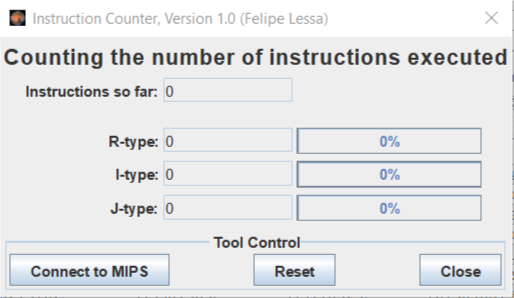
\includegraphics[width=7cm]{Images/IC.png}
		\end{center}
	\end{figure}
\end{center}
Sử dụng công thức sau để tính thời gian chạy:
\begin{center}
	$\text{CPU time} = \dfrac{\text{CPU Clock cycles}}{\text{Clock rate}}$ = $\dfrac{\text{Instruction Count x CPI}}{\text{Clock rate}}$
\end{center}
Trong đó:
\begin{itemize}
	\item CPU time là thời gian xử lý của chương trình (không tính thời gian giao tiếp I/O, thời gian chờ ...).
	\item CPU Clock cyles: Tổng số chu kỳ thực thi.
	\item Instruction Count là tổng số lệnh thực thi của chương trình.
	\item CPI (cycle per instruction) là số chu kỳ thực thi trên một lệnh.
	\item Clock rate là số chu kỳ thực thi trên một giây hay còn gọi là tần số, ví dụ: 4GHz = trong một giây có $4\text{x}10^9$ giao động.
\end{itemize}
Tuỳ vào cách bạn nhập mảng và nội dung mảng số mà chương trình có tổng số lệnh, loại lệnh và thời gian chạy khác nhau. Dưới đây là một số ví dụ cho thấy thời gian chạy khác nhau:
\subsection{Ví dụ 1}
Mảng nhập vào: [-17.6 -91.0 -18.8 27.7 85.8 -38.4 35.5 -13.2 -19.3 -73.0 24.3 -80.0 90.0 39.0 4.6 -82.0 41.0 70.0 -90.0 -13.2]\\
Tổng số lệnh: 3470\\
Trong đó:
\begin{itemize}
	\item R-type: 1345 lệnh chiếm 38\%
	\item I-type: 1927 lệnh chiếm 55\%
	\item J-type: 198 lệnh chiếm 5\%
\end{itemize}
Tính toán thời gian chạy:\\
$\text{CPU time} = \dfrac{\text{Instruction Count x CPI}}{\text{Clock rate}} = \dfrac{3400\text{x}1}{2\text{x}10^9} = 1.735 \text{x}10^{-6} s = 1.735 \mu s$
\subsection{Ví dụ 2}
Mảng nhập vào: [1.5 -3.2 4.5 -6.8 9.8 2.3 0.0 1.0 3.0 6.8 90.0 -100.0 156.0 79.0 -65.0 89.0 236.0 -5.0 6.0 56.0]\\
Tổng số lệnh: 3542\\
Trong đó:
\begin{itemize}
	\item R-type: 1375 lệnh chiếm 38\%
	\item I-type: 1983 lệnh chiếm 55\%
	\item J-type: 184 lệnh chiếm 5\%
\end{itemize}
Tính toán thời gian chạy:\\
$\text{CPU time} = \dfrac{\text{Instruction Count x CPI}}{\text{Clock rate}} = \dfrac{3400\text{x}1}{2\text{x}10^9} = 1.771 \text{x}10^{-6} s = 1.771 \mu s$
\subsection{Ví dụ 3}
Mảng nhập vào bằng cách Ramdom mảng: [-28.801712 92.848206 97.89546 -66.22838 -56.985153 -7.4053497 42.824326 73.07504 10.617569 -79.36971 62.384277 4.974922 76.675186 68.90369 -51.92387 5.409561 -0.9207001 37.36792 52.055145 8.778427 ]\\
Tổng số lệnh: 3400\\
Trong đó:
\begin{itemize}
	\item R-type: 1332 lệnh chiếm 39\%
	\item I-type: 1876 lệnh chiếm 55\%
	\item J-type: 192 lệnh chiếm 5\%
\end{itemize}
Tính toán thời gian chạy:\\
$\text{CPU time} = \dfrac{\text{Instruction Count x CPI}}{\text{Clock rate}} = \dfrac{3400\text{x}1}{2\text{x}10^9} = 1.7 \text{x}10^{-6} s = 1.7 \mu s$
\section{Code c++}
\begin{lstlisting}
#include <iostream>
#include <random>
#define NUMBER 19
#define Maxrand 100.0

using namespace std;

void swap(float data[], int a, int b) {
	float temp = data[a];
	data[a] = data[b];
	data[b] = temp;
}
void printArray(float data[], int low, int high) {
	for (int i = low; i <= high; i++) {
		cout << data[i] << " ";
	}
	cout << endl;
}
void quickSort(float Data[], int l, int r) {
	if (l <= r) {
		float key = Data[(l + r) / 2];
		int i = l;
		int j = r;
		while (i <= j) {
			while (Data[i] < key)
				i++;
			while (Data[j] > key)
				j--;
			if (i <= j) {
				swap(Data, i, j);
				i++;
				j--;
			}
		}
		if (l < j)
			quickSort(Data, l, j);
		if (r > i)
			quickSort(Data, i, r);
	}
}
int main() {
	int nhap;
	cout << "1. Nhap vao mang." << endl
		<< "2. Ramdom mot mang." << endl
		<< "Lua chon phuong an: ";
	cin >> nhap;
	float data[NUMBER + 1];
	switch (nhap) {
		case 1: {
			int i = 0;
			while (i <= NUMBER) {
				cout << "Nhap vao phan tu thu " << i << ": ";
				cin >> data[i];
				i++;
			}
			break;
		}
		case 2: {
			int i = 0;
			srand(time(NULL));
			while (i <= NUMBER) {
				data[i] = -Maxrand + (Maxrand + Maxrand) * rand() / RAND_MAX;
				i++;
			}
			break;
		}
		default:
			cout << "Ban lua chon sai!" << endl;
	}
	cout << "Mang cua ban truoc khi su dung quickSort:" << endl;
	printArray(data, 0, NUMBER);
	quickSort(data, 0, NUMBER);
	cout << "Mang cua ban sau khi su dung quickSort:" << endl;
	printArray(data, 0, NUMBER);
	return 0;
}
\end{lstlisting}

\newpage
%%%%%%%%%%%%%%%%%%%%%%%%%%%%%%%%%
%\addcontentsline{toc}{section}{Tài liệu tham khảo}
\begin{thebibliography}{99999}
	\bibitem{notes} MIPS Technologies, Inc {\em MIPS32™ Architecture For Programmers Volume II: The MIPS32™ Instruction Set.}  2003.
	\bibitem{vietcodes} {Hợp ngữ MIPS: \url{https://vietcodes.github.io/algo/mips}}.
	\bibitem{wiki}{ Sắp xếp nhanh: \url{https://vi.wikipedia.org/wiki/S%E1%BA%AFp_x%E1%BA%BFp_nhanh}}.
	\bibitem{geeksforgeeks}{ QuickSort: \url{https://www.geeksforgeeks.org/quick-sort/}}.
	
\end{thebibliography}

\end{document}

